\begin{tikzpicture}
  [
  vertex/.style={
    circle,
    fill=black,
    minimum size=1mm,
    inner sep=0pt
  },
  ->-/.style={
    decoration={
      markings,
      mark=at position 0.5 with {\arrow{#1}}
    },
    postaction={decorate}
  }
  ]
  \node at (0,0) [vertex] {}
  edge [->-={>}] (1,0)
  node at (1,0) [vertex] {}
  edge [->-={<}] (1,1)
  node at (1,1) [vertex] {}
  edge [->-={<<}] (0,1)
  node at (0,1) [vertex] {}
  edge [->-={>>}] (0,0);
  \node at (2.5,0) [vertex] {};
  \draw (2.5,0) to [out=45,in=135,loop] (2.5,0);
  \node at (2,1) [vertex] {}
  edge [bend right] (3,1)
  node at (3,1) [vertex] {}
  edge [bend right] (2,1);
\end{tikzpicture}
\hspace{1cm}
\begin{tikzpicture}
  [
  vertex/.style={
    circle,
    fill=black,
    minimum size=1mm,
    inner sep=0pt
  },
  ->-/.style={
    decoration={
      markings,
      mark=at position 0.5 with {\arrow{#1}}
    },
    postaction={decorate}
  }
  ]
  \node at (0,0) [vertex] {}
  edge [->-={>}] (1,0)
  node at (1,0) [vertex] {}
  edge [->-={<}] (2,0)
  node at (2,0) [vertex] {}
  edge [->-={<<}] (2,1)
  node at (2,1) [vertex] {}
  edge [>={Stealth},->-={>}] (1,1)
  node at (1,1) [vertex] {}
  edge [>={Stealth},->-={<}] (0,1)
  node at (0,1) [vertex] {}
  edge [->-={>>}] (0,0);
  \draw (1,0) -- (1,1);

  \node[shift={(3,0)}] at (0,0) [vertex] {}
  edge [shift={(3,0)},bend left] (1,0)
  node [shift={(3,0)}] at (1,0) [vertex] {}
  edge [shift={(3,0)},bend left] (0,0);
\end{tikzpicture}
\ \\\vspace{.5cm}
% Sphere
\begin{tikzpicture}
  [
  vertex/.style={
    circle,
    fill=black,
    minimum size=1mm,
    inner sep=0pt
  },
  ->-/.style={
    decoration={
      markings,
      mark=at position 0.5 with {\arrow{#1}}
    },
    postaction={decorate}
  }
  ]
  \node ( 1) at ( 0, 0) [vertex] {};
  \node ( 2) at ( 0, 1) [vertex] {};
  \node ( 3) at ( 1, 0) [vertex] {};
  \node ( 4) at ( 1, 1) [vertex] {};
  \node ( 5) at ( 0, 2) [vertex] {};
  \node ( 6) at ( 1, 2) [vertex] {};
  \node ( 7) at ( 0, 3) [vertex] {};
  \node ( 8) at ( 1, 3) [vertex] {};
  \node ( 9) at (-1, 1) [vertex] {};
  \node (10) at (-1, 2) [vertex] {};
  \node (11) at ( 2, 1) [vertex] {};
  \node (12) at ( 2, 2) [vertex] {};
  \node (13) at ( 3, 1) [vertex] {};
  \node (14) at ( 3, 2) [vertex] {};
  \draw[->-=>] (0,0) -- (1,0);
  \draw[->-=>>] (1,0) -- (1,1);
  \draw[->-=<<] (1,1) -- (2,1);
  \draw[->-=<] (2,1) -- (3,1);
  \draw[>={Stealth}, ->-=>] (3,1) -- (3,2);
  \draw[>={Stealth}, ->-=<<] (3,2) -- (2,2);
  \draw[>={triangle 45}, ->-=>] (2,2) -- (1,2);
  \draw[>={triangle 45}, ->-=<] (1,2) -- (1,3);
  \draw[>={Stealth}, ->-=>>] (1,3) -- (0,3);
  \draw[>={triangle 45}, ->-=<<] (0,3) -- (0,2);
  \draw[>={triangle 45}, ->-=>>] (0,2) -- (-1,2);
  \draw[>={Stealth}, ->-=<] (-1,2)-- (-1,1);
  \draw[>={open triangle 45}, ->-=>] (-1,1) -- (0,1);
  \draw[>={open triangle 45}, ->-=<] (0,1) -- (0,0);
  \draw (0,1) -- (1,1) -- (1,2) -- (0,2) -- (0,1);
  \draw (2,2) -- (2,1);
\end{tikzpicture}
% link of sphere
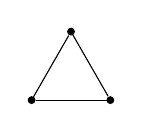
\begin{tikzpicture}
  [
  vertex/.style={
    circle,
    fill=black,
    minimum size=1mm,
    inner sep=0pt
  }]
  \node at (0,0) [vertex] {}
  edge (1,0)
  node at (1,0) [vertex] {}
  edge (0.5, 0.87)
  node at (0.5, 0.87) [vertex] {}
  edge (0,0);
\end{tikzpicture}

%%% Local Variables:
%%% mode: latex
%%% TeX-master: "../Master"
%%% End:
